\documentclass[11pt]{article}
\usepackage[margin=1in]{geometry}
\usepackage{amsmath,amssymb,booktabs,tabularx,graphicx}
\usepackage[hidelinks]{hyperref}
\usepackage[T1]{fontenc}
\title{Digital Twin Technology for River Basin Management:\\
An Availability-Aware Decision-Support Prototype}
\author{Working research manuscript}
\date{27 October 2026}
\begin{document}
\maketitle
\begin{center}
\fbox{\parbox{0.92\linewidth}{\textbf{Research status.} This is an implementation and exploratory-results draft, not a submission-ready validated study. Satellite modules have been implemented and tested offline; real satellite exports, independent reference data, and a verified agricultural study basin are outstanding.}}
\end{center}

\begin{abstract}
River-basin decision support must distinguish an observation's acquisition period from the time when that observation becomes available. We implement a modular prototype that links satellite-derived agricultural and hazard indicators, probabilistic streamflow forecasts, and constrained water-allocation scenarios through an availability-aware state interface. The observation modules include dual-polarization Sentinel-1 rice classification, MODIS thermal--optical trapezoid surface wetness, SAR flood and slope-change screening, and an optical turbidity index. Each module has an explicit interpretation and validation boundary. Missing or stale crop and wetness observations trigger abstention rather than a zero-demand estimate. An exploratory replay uses 2,192 archived Potomac River daily forecasts with hypothetical demand, environmental reserve, and abstraction constraints. A lower-tail forecast policy reduces supply overcommitment relative to mean-forecast planning, but increases unmet hypothetical demand. This tradeoff demonstrates the decision-evaluation workflow; it does not establish satellite benefit, operational water savings, or transfer to another basin. We specify the spatial, temporal, and observation-latency experiments required to test those claims.
\end{abstract}

\section{Introduction}
Digital twins for river basins already integrate observations, models, scenarios, and stakeholder-facing decisions \cite{yang,iwmi}. An additional dashboard or collection of remote-sensing maps is therefore insufficient to establish a new scientific contribution. A more specific question is whether information improves a defined decision under realistic constraints on its quality and availability.

This prototype addresses the question: \emph{Under which observation-error and latency conditions do crop and surface-moisture observations improve water-allocation outcomes relative to flow-only information, and when should a system abstain?} This question remains to be answered empirically using real satellite and independent reference observations. The current work contributes an executable evaluation structure and a preliminary flow-based decision replay.

Three distinctions guide the implementation. First, a surface-wetness index is not a measured root-zone moisture state. Second, a retrospective composite is not available at the start of its observation interval. Third, higher forecast skill does not automatically imply a preferable allocation policy. These distinctions motivate separate validation of observation products, forecasts, and decision outcomes.

\section{Study context and available evidence}
The existing research repository contains a single-station streamflow benchmark for USGS station 01646500, Potomac River near Washington, DC \cite{usgs}. The archived response covers 1990--2025. The existing benchmark uses 1990--2009 for model fitting, 2010--2014 for validation, 2015--2019 for forecast-mixture calibration, and 2020--2025 for testing. The final period contains 2,192 rolling next-day forecasts.

The model suite comprises an LSTM, stacked LSTM, bidirectional LSTM, Transformer, persistence, equal averaging, and calibrated forecast Bayesian model averaging (BMA). BMA here denotes an empirically calibrated forecast mixture, not a full Bayesian posterior over neural-network parameters. The present extension consumes saved forecasts without refitting those models.

The Potomac is the existing flow test site; it has not been established as the appropriate paddy-study basin. No verified crop-reference dataset, basin boundary for the proposed satellite experiment, paired soil-moisture measurements, or real satellite output is included in the current evaluation. A separate constructed-wetland dataset in the repository is not used.

\section{Observation-to-decision framework}
The workflow comprises four stages:
\begin{enumerate}
\item Extract quality-screened observations with spatial support, observation-interval end, source identity, and release/vintage metadata.
\item Fit or apply observation modules using partitions appropriate to their intended use.
\item Form a management-unit state from observations available by the decision issue time.
\item Evaluate constrained allocation scenarios and record missing-data abstentions and candidate-hazard review flags.
\end{enumerate}
The implementation is a research prototype rather than a fully synchronized operational basin twin. It does not yet include channel routing, a reservoir operating model, groundwater coupling, automatic sensor ingestion, or field actuator feedback.

\subsection{Rice classification from Sentinel-1}
Sentinel-1 GRD observations are filtered to a common instrument mode, pass, relative orbit, resolution and VV/VH polarization set, following the official preprocessing guidance \cite{s1}. Monthly VV and VH summaries and their temporal sequences form a baseline feature vector. The polarization contrast is
\begin{equation}
r_{\mathrm{dB}}=\sigma^0_{\mathrm{VV,dB}}-\sigma^0_{\mathrm{VH,dB}},
\end{equation}
which is a log power ratio; division of two dB values is not used.

The offline classifier uses training-only median imputation and a random forest with 200 trees, minimum leaf size three and balanced class weights. A fixed seed supports reproducibility. Training and evaluation spatial groups must be disjoint. The supplied command evaluates retrospective end-of-season classification; an in-season claim would require separately trained prefix models and documented training-label availability.

Outputs include rice probability, F1, balanced accuracy, average precision, Brier score and a confusion matrix. Forest probabilities are not asserted to be calibrated uncertainty. Evaluation with map-derived labels alone measures agreement with that map; independent field references are needed for a field-accuracy claim. Management-unit crop fractions require documented area-weighted aggregation and uncertainty analysis.

\subsection{MODIS surface-wetness baseline}
The thermal--optical trapezoid model (TOTRAM) estimates relative surface wetness from a pixel's location between wet and dry edges in vegetation-index--temperature space \cite{trapezoid,sadeghi}. For vegetation index $v$, let
\begin{equation}
T_{\mathrm{wet}}(v)=a_w+b_wv,\qquad
T_{\mathrm{dry}}(v)=a_d+b_dv.
\end{equation}
The relative index is
\begin{equation}
W=\frac{T_{\mathrm{dry}}(v)-T}{T_{\mathrm{dry}}(v)-T_{\mathrm{wet}}(v)}.
\end{equation}
The implementation estimates conditional 5th and 95th temperature percentiles in NDVI bins, fits linear edges, and rejects scenes with inadequate vegetation range, insufficient populated bins, or crossing/insufficiently separated edges. Outputs retain the unclipped index and identify values outside the fitted edges; clipping to $[0,1]$ is not concealed.

MOD13A2 vegetation indices and MOD11A2 temperature are quality screened and scaled using their documented conventions \cite{modis}. Complete 8-day temperature composites are matched within a 16-day vegetation interval. This is an approximate composite pairing, not simultaneous acquisition. Computation retains approximately 1 km support. Resampling does not create field-scale information.

Fitting is scene-specific with an initial 200 m elevation stratification. This does not establish homogeneous weather or adequate wet/dry coverage; those assumptions require diagnosis. $W$ is a dimensionless surface indicator and is not converted to volumetric or root-zone moisture without independent calibration.

\subsection{Flood, turbidity and slope-change screening}
The flood baseline identifies substantial SAR darkening combined with low post-event backscatter, low slope, and exclusion of persistent water. Small connected components are removed. Starting thresholds are a 3 dB drop, post-event backscatter at most $-15$ dB, slope at most $5^\circ$, and eight connected pixels. These are configurable controls, not validated site-specific values. The approach follows the family of SAR flood-change practices described by UN-SPIDER \cite{flood}; it can omit inundation in vegetation, cities and double-bounce settings.

For cloud-screened water pixels, the normalized difference turbidity index is
\begin{equation}
\mathrm{NDTI}=\frac{\rho_{\mathrm{red}}-\rho_{\mathrm{green}}}
{\rho_{\mathrm{red}}+\rho_{\mathrm{green}}}.
\end{equation}
It remains an index. No NTU, suspended-solids concentration or water-safety interpretation is assigned without paired measurements and an appropriate calibration \cite{turbidity}.

Slope-change screening identifies absolute before/after SAR changes of at least 4 dB on slopes of at least $15^\circ$, subject to component filtering. Such change is not specific to landslides. The output is a candidate-review layer, not a landslide inventory, deformation measurement or forecast. Published amplitude-based research similarly identifies limitations in mapping landslide boundaries \cite{landslide}. Terrain layover/shadow and radiometric effects require dedicated treatment before mountainous-basin validation.

\subsection{Availability-aware state and abstention}
Each record contains a unit identifier, variable, observation-support end $t_o$, availability time $t_a$, value and source identifier. At issue time $t$, an observation is eligible only if
\begin{equation}
t_o\leq t_a\leq t,\qquad 0\leq t-t_o\leq \Delta_{\max}.
\end{equation}
The latest eligible observation and release vintage are retained per unit and variable. Ambiguous duplicate vintages are rejected. An observation known only after the issue time cannot enter the decision, even if its acquisition period predates that time.

If crop fraction or surface wetness is missing or stale, the connected planner abstains. Optional flood and slope-change fractions create review flags. Turbidity does not automatically prohibit allocation because a calibrated water-quality threshold is absent. The current Earth Engine exports explicitly identify historical availability as unverified; operational replay requires actual release/vintage records or declared latency assumptions.

\subsection{Allocation and physical accounting}
For hypothetical management-unit area $A_i$ in hectares, rice fraction $p_i$, wetness $W_i$, dry-condition demand depths $d_r,d_o$, response coefficient $\alpha$ and delivery efficiency $\eta$, the scenario demand is
\begin{equation}
D_i=\frac{10A_i}{\eta}\,[p_id_r+(1-p_i)d_o](1-\alpha W_i).
\end{equation}
The factor 10 converts hectare-millimetres to cubic metres. This is a transparent sensitivity model, not a validated crop-water requirement; surface wetness cannot directly substitute for root-zone water availability.

Given forecast supply quantile $q_\tau$, reserve $q_e$, abstraction fraction $f$ and interval $\Delta t$, the supply budget is
\begin{equation}
B=f\,\Delta t\,\max(q_\tau-q_e,0),\qquad
a_i=D_i\min\left(1,\frac{B}{\sum_jD_j}\right).
\end{equation}
This proportional-shortage rule is a baseline rather than an optimization of legal rights, crop yield or economic welfare. A separate single-bucket module enforces
\begin{equation}
S_{t+1}=S_t+P_t+I_t-R_t-ET_t
\end{equation}
with bounded storage and water-limited evapotranspiration. It is not a paddy-ponding or distributed basin model.

\section{Exploratory decision replay}
The replay compares persistence, BMA mean, and the lower endpoint of the archived BMA 90\% interval (the 5th percentile). For all policies, hypothetical demand is 3 million m$^3$/day, divided equally among three units; the reserve is 20 m$^3$/s and the diversion cap is 10\% of flow above that reserve. These numbers are scenario assumptions, not calibrated Potomac demand, policy or legal entitlements.

Planned allocation uses forecasts only. Observed daily discharge subsequently determines feasible delivery and supply overcommitment. Observations do not enter the decision rule. Overcommitment is planned volume above the observed scenario budget; it is not evidence that an actual abstraction occurred.

\begin{table}[ht]
\centering
\small
\begin{tabular}{lrrr}
\toprule
Policy & Overcommitment & Mean unmet demand & Mean overcommitment\\
 & days (\%) & (million m$^3$/day) & (m$^3$/day)\\
\midrule
Persistence & 54.47 & 1.5893 & 63,317\\
BMA mean & 63.55 & 1.5688 & 78,526\\
BMA 5th percentile & 1.46 & 1.8381 & 2,717\\
\bottomrule
\end{tabular}
\caption{Exploratory results over 2,192 days. Flow observations and forecasts are archived data; demands and policy constraints are hypothetical. No satellite observations enter this replay.}
\label{tab:replay}
\end{table}

Table~\ref{tab:replay} shows a tradeoff rather than universal superiority. Conservative planning produces fewer supply overcommitments while withholding more potentially deliverable water. The BMA mean policy leaves slightly less demand unmet than persistence but overcommits on more days. Consequently, model selection using prediction error alone would not specify an allocation preference. These findings are conditional on the scenario and previously inspected test period; they are not a new confirmatory test of the forecasting models.

\begin{figure}[ht]
\centering
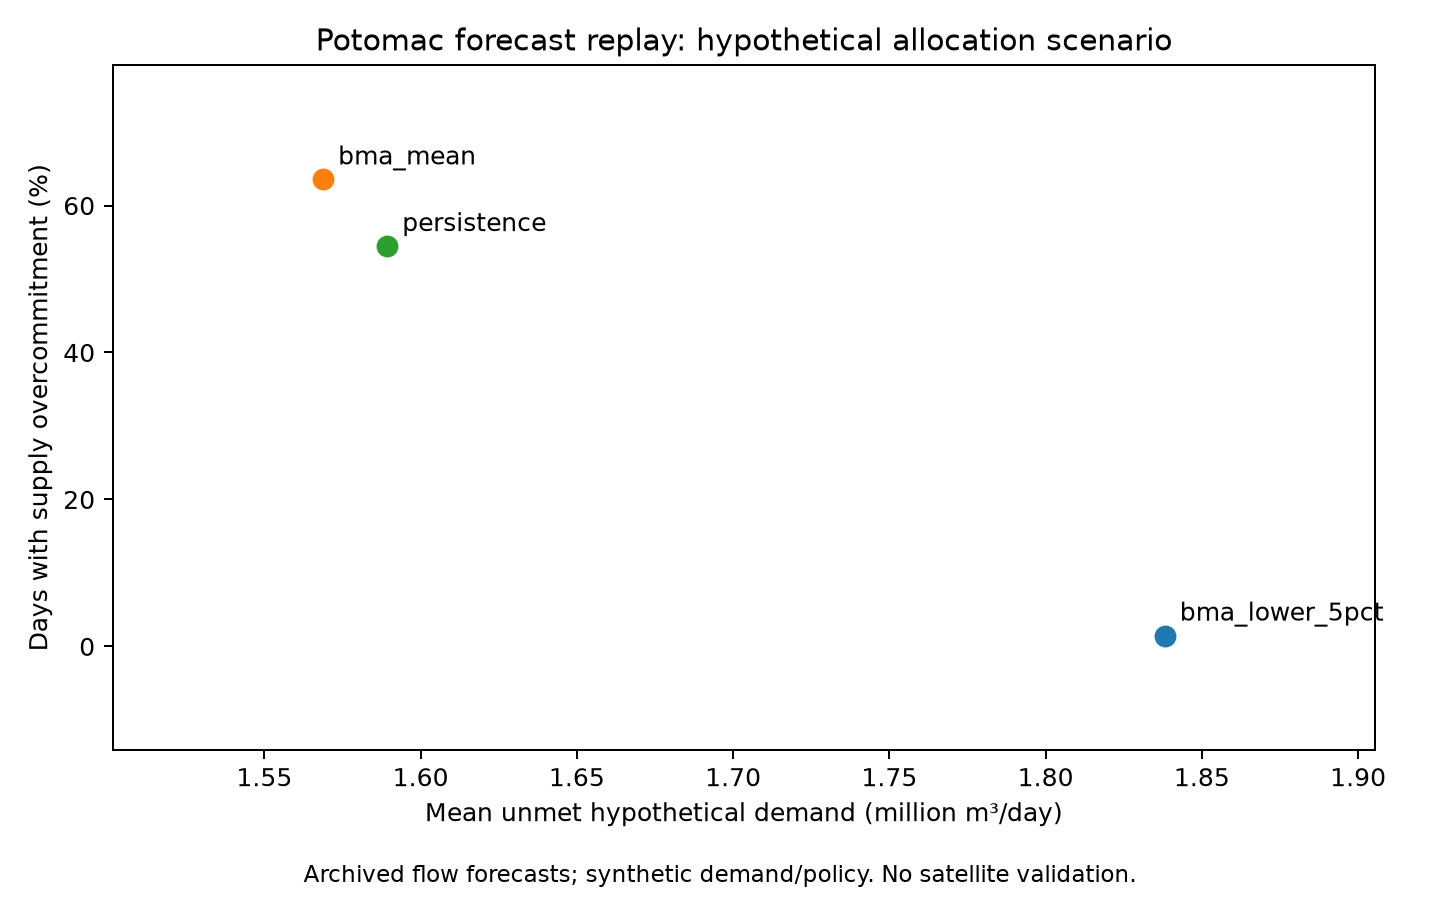
\includegraphics[width=\linewidth]{images/decision_tradeoff.png}
\caption{Allocation tradeoff under the single hypothetical scenario. Independent satellite validation and uncertainty intervals for cross-scenario conclusions are still required.}
\end{figure}

\section{Experiments required for a substantive research claim}
The intended novelty must be assessed against a fuller literature review and established by evidence. The following experiments define a focused path:
\begin{enumerate}
\item \textbf{Crop and moisture ablations.} Compare full information, fixed crop fractions, absent moisture response, and flow-only planning under identical constraints.
\item \textbf{Latency and missingness.} Evaluate measured availability first, then additional 3/7/14/30-day delays and structured cloud/sensor outages. Report decision-loss and abstention curves together.
\item \textbf{Calibrated uncertainty.} Propagate empirically measured crop, edge and forecast errors with spatial dependence. Uncalibrated forest scores must not be treated as posterior samples.
\item \textbf{Transfer and independence.} Hold out buffered spatial blocks, seasons, events and catchments; reserve new untouched evaluation data. Use train-only calibration and several prespecified seeds.
\item \textbf{Decision outcomes.} Report unmet demand, supply overcommitment, reserve violations, distribution across units and regret against a clearly defined perfect-information bound.
\end{enumerate}
Paired block-bootstrap intervals should account for hydrological dependence. Neighboring pixels and consecutive days must not be treated as independent replications. Thresholds and hyperparameters should be selected within training/validation partitions rather than against final event outlines.

Rice maps need independent reference labels and sampling design. Wetness estimates require depth-, footprint- and time-matched field observations; coarse products may provide comparison but not field-scale ground truth. Flood and landslide layers need independent event inventories. Turbidity requires paired laboratory or sensor measurements and held-out water bodies/events. These validations are prerequisites for claims about the value of each module.

\section{Reproducibility and limitations}
Code is organized into observation kernels, satellite export/pipeline commands, an availability-aware state/decision module, and an archived-forecast replay. Input SHA-256 hashes, output tables and separate dependency locks support auditability. Existing model predictions are retained unchanged. Offline tests cover chronology, spatial-group leakage, scale/quality masks, degenerate edge fits, component screening, units, budgets, abstention and water balance. Synthetic test fixtures validate software behavior only.

Earth Engine scripts have been syntax-checked but not remotely executed. No real satellite mapping accuracy or field-scale performance is reported. The present work lacks a verified agricultural study boundary, matched satellite/reference data, flow routing, reservoir dynamics, calibrated crop demand, actual governance constraints and a prospective deployment. It should therefore be described as an executable prototype and an exploratory decision evaluation, not a completed operational digital twin.

\section{Conclusion}
The implementation makes observation availability, interpretation and missingness explicit at the interface between satellite indicators and allocation scenarios. The existing-flow replay demonstrates why conservative supply planning and demand satisfaction must be assessed jointly. Establishing a distinctive research contribution now requires the specified independent satellite and decision-value experiments; the current results do not justify claims of satellite-driven water savings or general superiority.

\begin{thebibliography}{10}
\raggedright
\bibitem{yang} Yang et al. (2024). Digital twinning of river basins towards full-scale, sustainable and equitable water management and disaster mitigation. \emph{npj Natural Hazards}. \url{https://doi.org/10.1038/s44304-024-00047-2}.
\bibitem{iwmi} International Water Management Institute. Digital twins. \url{https://www.iwmi.org/topics/digital-twins/}. Accessed 27 October 2026.
\bibitem{usgs} U.S. Geological Survey. Monitoring location USGS-01646500. \url{https://waterdata.usgs.gov/monitoring-location/USGS-01646500/}. Archived daily-value response retrieved 8 October 2026.
\bibitem{s1} Google Earth Engine. Sentinel-1 algorithms. \url{https://developers.google.com/earth-engine/guides/sentinel1}.
\bibitem{trapezoid} A Comparison of Three Trapezoid Models Using Optical and Thermal Satellite Imagery for Water Table Depth Monitoring in Estonian Bogs (2020). \emph{Remote Sensing}, 12(12), 1980. \url{https://www.mdpi.com/2072-4292/12/12/1980}.
\bibitem{sadeghi} Sadeghi et al. (2017). The optical trapezoid model: A novel approach to remote sensing of soil moisture applied to Sentinel-2 and Landsat-8 observations. \emph{Remote Sensing of Environment}. \url{https://www.sciencedirect.com/science/article/pii/S0034425717302493}.
\bibitem{modis} Google Earth Engine Data Catalog. MOD13A2.061 and MOD11A2.061. \url{https://developers.google.com/earth-engine/datasets/catalog/MODIS_061_MOD13A2}; \url{https://developers.google.com/earth-engine/datasets/catalog/MODIS_061_MOD11A2}.
\bibitem{flood} UN-SPIDER. Recommended practice: Flood mapping and damage assessment using Sentinel-1 SAR data in Google Earth Engine. \url{https://un-spider.org/advisory-support/recommended-practices/recommended-practice-google-earth-engine-flood-mapping/in-detail}.
\bibitem{turbidity} A Comparison of Non-Contact Methods for Measuring Turbidity in the Colorado River (2026). \emph{Remote Sensing}, 18(4), 638. \url{https://www.mdpi.com/2072-4292/18/4/638}.
\bibitem{landslide} Sentinel-1 SAR Amplitude Imagery for Rapid Landslide Detection (2019). \emph{Remote Sensing}, 11(7), 760. \url{https://www.mdpi.com/2072-4292/11/7/760}.
\end{thebibliography}
\end{document}
